\documentclass{swim}
\usepackage{geometry}
\usepackage{tikz}
\geometry{
 letterpaper,
 total={7.5in,10in},
}

\tracingoutput=1
\showboxdepth=3
\showboxbreadth=99

\title{Swim}
\author{Karlie Meads}

\begin{document}
\vbox{
\begin{minipage}[t][0.5\textheight][t]{0.95\textwidth}
\tikz[remember picture,overlay]
  \node[anchor=north east,inner sep=25pt] at (current page.north east)
    {\includegraphics[width=0.4\textwidth]{Greenbrittlestar.png}};
\section{Brittle Star: 2300m\\}

https://www.swimdojo.com/workouts/2021/3/29/brittle-star

\subsection{Warm Up: 700}
\begin{itemize}
  \item 200 swim
  \item 300 K/D/S IM order by 25
  \item 4 $\times$ 50 stroke $\rightarrow$ drill down, swim back @ :15 rest
\end{itemize}


\subsection{Main Set: 1400}
\begin{itemize}
    \item 4 $\times$ 50 stroke @ stroke base (aka sb $\rightarrow$ this will vary depending on which stroke you are doing and ability level)
    \item 2 $\times$ 100 free @ b +5
    \item 3 $\times$ 100 stroke FAST @ sb +15
    \item 2 $\times$ 100 free @ b +5
    \item 2 $\times$ 100 stroke FAST @ sb +15
    \item 2 $\times$ 100 free @ b +5
    \item 100 stroke FAST @ sb +15
\end{itemize}

\subsection{Warm Down: 200}
200 easy

Notes: For the stroke on this set you can do IM if you’d prefer. To figure out your stroke base, do a 50 at a comfortable pace and add 10 seconds.
\end{minipage}

\nointerlineskip
\begin{minipage}[b][0.5\textheight][t]{0.95\textwidth}
  \vspace{0.4in}

\tikz[remember picture,overlay]
  \node[anchor=north east,inner sep=25pt] at (current page.east)
    {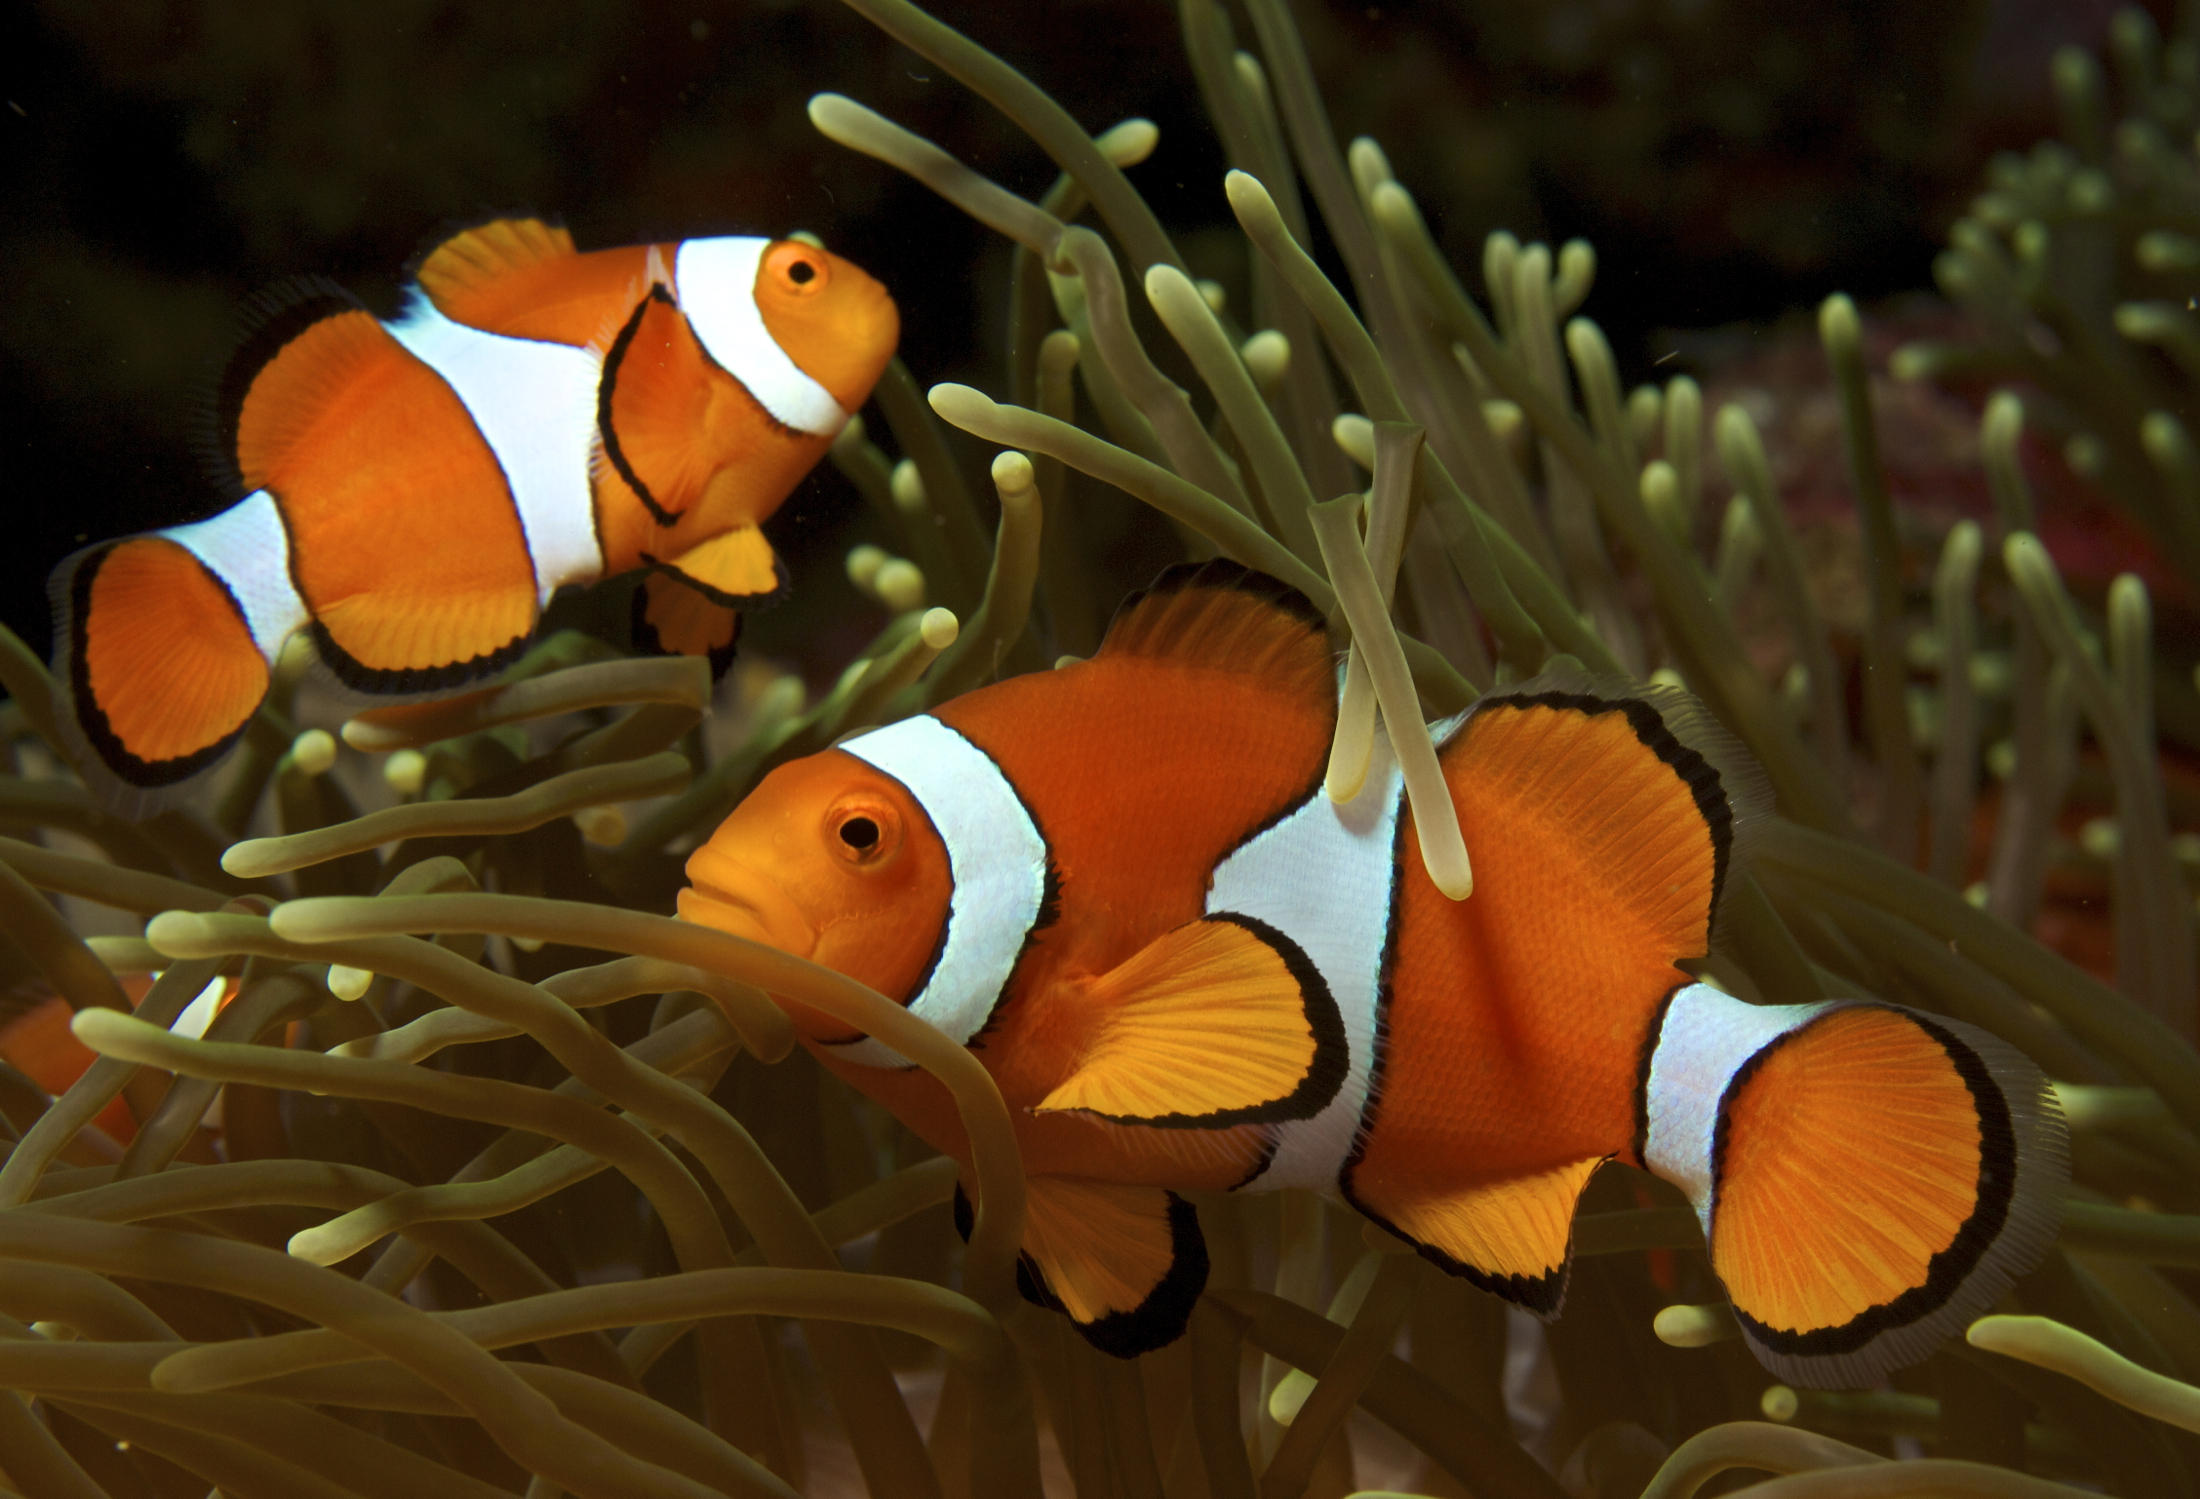
\includegraphics[width=0.4\textwidth]{Clownfish.jpg}};
\section{Clownfish: 2000m\\}

https://www.swimdojo.com/workouts/2019/9/19/clownfish

\subsection{Warm Up: 600}
\begin{itemize}
  \item 200 choice
  \item 8 x 50 @ 10 seconds rest —>odds kick, evens swim
\end{itemize} 

\subsection{Set 1: 650}
\begin{itemize}
  \item 100 free @ b +5
  \item 6 x 25 stroke @ :30 (or slower base if needed)
  \item 100 free @ b+5
  \item 6 x 50 stroke @ b+20
\end{itemize} 

\subsection{Set 2: 600}
\begin{itemize}
  \item 4 x 100 kick @ kb
  \item 8 x 25 @ :30
  \item —>4x: 25 only two breaths, 25 half sprint half easy, 25 only 2 breaths, 25 half easy half sprint
\end{itemize}  

\subsection{Warm Down: 150}
\begin{itemize}
  \item 100 easy
\end{itemize} 

Notes: This is a variation of the Terrible Claw Lobster workout. Remember on stroke workouts to adjust bases as needed depending on your ability level. The bases should be challenging but doable, don’t let your stroke completely fall apart as you get tired.
Of the over 1,000 anemone species that live in the ocean, only 10 species coexists with the 26 species of tropical clownfish. All clownfish are born as males. When the dominant female of a group dies the largest male will turn itself into a female, this change cannot be reversed back. 


\end{minipage}}
\end{document}
